\section{Systementwurf}
\textcolor{red}{Lorem ipsum dolor sit amet, consetetur sadipscing elitr, sed diam nonumy eirmod tempor invidunt ut labore et dolore magna aliquyam erat, sed diam voluptua. Lorem ipsum dolor sit amet, consetetur sadipscing elitr, sed diam nonumy eirmod tempor invidunt ut labore et dolore magna aliquyam erat, sed diam voluptua. Lorem ipsum dolor sit amet, consetetur sadipscing elitr, sed diam nonumy eirmod tempor invidunt ut labore et dolore magna aliquyam erat, sed diam voluptua. Lorem ipsum dolor sit amet, consetetur sadipscing elitr, sed diam nonumy eirmod tempor invidunt ut labore et dolore magna aliquyam erat, sed diam voluptua.}

\subsection{Vorgehensweise Anforderungserhebung}
Die Anforderungen für das zu konzipierende System wurden vor dem Hintergrund der Evaluation des Prozesses erhoben. Außerdem wurde bei der Erfassung der Anforderung darauf geachtet, das der Prototyp beim Praxispartner als Unterstützung für zukünftige Innovationsfragen herangezogen werden soll. Wie von \citet{Dick2017, HullElizabeth2011} beschrieben, kann das Prototyping selbst bereits als Anforderungsanalyse angesehen werden, jedoch wurde für die prototypische Implementierung des Systementwurfs eine gesonderte Anforderungsanalyse durchgeführt. Ziel dieser Vorgehensweise ist eine präzise Definition und Eingrenzung der Anforderungsbeschreibung während des Konzeptions- und Implementierungsprozesses.

Im Zuge der Anforderungserhebung wurden die Anforderungen in Zusammenarbeit mit dem Praxispartner entwickelt. Die Anforderungen wurden dabei in textueller Form nach einem festen Muster in Anlehnung an \citet{PohlKlaus2015} definiert. Ergänzt wurden die textuellen Anforderungen um Prozessdiagramme und Mockups der Nutzeroberflächen. Der Fokus des konzipierten System liegt dabei allerdings auf eigentlichen Blockchain Netzwerk und weniger auf der Benutzeroberfläche.

Die Anforderungen wurden untergliedert in funktionale Anforderungen, Rahmenbedingungen und Qualitätsanforderungen. Ebenso wurden die Anforderungen hierarchisiert und um eine Quelle ergänzt \citep{Koelsch2016}. Dies soll die Nachverfolgbarkeit der Anforderungen während der Evaluation unterstützen.

\subsection{Das Ziel: Chargenrückverfolgung innerhalb der Fleischwarenindustrie} \label{goal-description}
Das System soll unter experimentellen Bedingungen die Chargenrückverfolgung von Schweinen innerhalb der Wertschöpfungskette realisieren. Dafür muss das System den Prozess vom Erzeuger bis zum Groß- und Einzelhandel unterstützen. Konkret sollen Erzeuger neue Tiere im Blockchain Netzwerk registrieren und zu einer Charge zuordnen können. Bereits registrierte Tiere sollen zur Weiterverarbeitung freigegeben werden können und ein Eigentumswechsel muss durch das System abgebildet werden können. Die Summe der Transaktionen zwischen den Teilnehmern der Wertschöpfungskette bildet schließlich einen Graphen. Anhand dieses Graphen soll eine Rückverfolgbarkeit einer Charge gewährleistet werden. Über eine Benutzeroberfläche sollen die Teilnehmer jederzeit in der Lage sein den Graphen einsehen zu können. Für die technische Umsetzung des System spielt die Benutzeroberfläche jedoch eine nachgelagerte Rolle. Hauptaugenmerk des Systementwurfs liegt auf dem technologischen Aufbau des Blockchain Netzwerk und seinen Schnittstellen für etwaige Drittsysteme zur automatischen Erfassung von Tieren. Eine automatische Erfassung von neuen Tieren kann beispielsweise über \ac{iot}-Sensoren erfolgen. Ebenso würde sich ein Eigentumswechsel, wenn Tiere vom Erzeuger an den Schlachthof verkauft werden, über RFID-Chips und entsprechende Lesegeräte welche per Schnittstelle mit dem Blockchain Netzwerk verbunden sind abwickeln lassen \citep{Dorri2017, Samaniego2016}.

\subsection{Die Wertschöpfungskette im Detail}
Nachfolgend soll eine kurze Erläuterung der in Kapitel \ref{goal-description} erwähnten Wertschöpfungskette dazu dienen, die Daten- und Warenströme zwischen den Teilnehmern klar zu trennen und die für diesen Systementwurf wichtigen Informationen herauszuarbeiten. Da eine Chargenrückverfolgung nur gewährleistet werden kann, wenn in den vorgelagerten Prozessen die nötigen Informationen in einem System bereitgestellt wurden, soll kurz auf die Teilschritte vom Erzeuger zum Endverbraucher eingegangen werden.

Die Fleischwirtschaft hat in den letzten Jahren einen Strukturwandel vollzogen, welcher auch Auswirkungen auf die eigentliche Tätigkeit sowie die Lieferanten- und Abnehmerbeziehungen zwischen den Unternehmen hat \citep{Nolte2006}. Als eine der zentralen Ursachen für den Strukturwandel wird die Konzentrierung der Schlachtunternehmen gezählt. Inzwischen werden deutlich mehr als 50\% aller Schweine in Deutschland von drei Unternehmen geschlachtet - Tönnies, Vion und Westfleisch. Unter Beachtung anderer Wirtschaftszweige wie beispielsweise der Geflügelschlachtung, die noch wesentlich stärker konzentriert ist, und dem Hintergrund das in Ländern wie Dänemark die Schlachtung nur noch von zwei Unternehmen durchgeführt wird, wird deutlich das der Konzentrationsprozess in Deutschland auf der Schlachtstufe noch nicht abgeschlossen ist. Im Gegensatz dazu ist der Viehandel und die Landwirtschaft weniger stark konzentriert, weshalb sie sich in einer schwachen Verhandlungsposition befinden. Um dieser schwachen Verhandlungsposition entgegenzuwirken sind Unternehmen des Viehandels dazu gezwungen immer größere Mengen an Schlachttieren zu einer Charge zu bündeln. Ebenfalls sind zahlreiche unternehmensübergreifende Kooperationen im Viehandel zu beobachten \citep{Voss2010}.

Vom Erzeuger bis zum Endverbraucher ist die Wertschöpfungskette in Deutschland sehr vielfältig ausgeprägt \citep{Freund1997}. Der Hauptabsatzweg für Schweinemäster läuft entweder über eine direkt Vermarktung an Schlachtbetriebe (einstufige Vermarktung) oder indirekt über den privaten Viehandel, Viehvermarktungsgenossenschaften oder Erzeugergemeinschaften (zweistufige Vermarktung). Die Schlachtstufe lässt sich daher als Flaschenhals der Wertschöpfungskette aus Sicht der Schweinemäster betrachten.

Die Wertschöpfungskette vom Erzeuger bis zum Fleischwarenproduzenten gliedert sich grob in fünf Schritte, welche nachfolgend kurz beschrieben und in Abbildung \ref{fig:value-chain-meat} schematisch dargestellt werden. Dabei sind vier Parteien direkt in den Gesamtprozess involviert und eine fünfte Partei wirkt indirekt als Vermittler zwischen den anderen Parteien mit.

1.1 Futtermittelbestellung\\
1.2 Futtermittellieferung\\
1.3 Meldung über Futtermittellieferung (DESADV optional)\\
2.1 Ferkellieferung\\
2.2 Aufnahmemeldung\\
3.1 Meldung schlachtreifer Schweine\\
3.2 Weitervermittlung schlachtreifer Schweine an Schlachthof\\
3.3 Lieferauftrag\\
3.4.1 elektronische Ankündigung der Schlachtviehlieferung\\
3.4.2 Schweinelieferung\\
3.4.3 Wareneingangsmeldung (optional)\\
4.1 Erfassung VVVO Landwirt, Vergabe Partie-Nr. je Lkw (individuell vom Schlachthof)\\
4.2 Aufbringen einer fortlaufenden Schlacht-Nr. (manuell)\\
4.3 Meldung Schlachtdaten\\
5.1 Bestellung Schweinehälften\\
5.2.1 u.a. Artikelbezeichnung, Stückzahl, Schlachtdatum, Schlacht-Nr., Schadenskennzeichen\\
5.2.2 Anlieferung Schweinehälften\\
5.3 Automatische Zubuchung Schweinehälfte und Gewicht, Automatische Verknüpfung mit Lieferschein im ERP-System\\

1. Textuelle Beschreibung der Wertschöpfungskette und des Geschäftsprozess der Chargenrückverfolgung inklusiver einem kleinen Ausschnitt der nötigen vor- und nachgelagerten Prozesse (Wareneingang/-ausgang, Eigentumsübertragung, Logistik)\\
2. Abbildung der Wertschöpfungskette und des Geschäftsprozess

\subsection{Rahmenbedingungen}
1. Alle Rahmenbedingungen textuell beschreiben und wo sie hergeleitet sind, immer mit Referenz auf die Tabelle in der die Übersicht aller Rahmenbedingungen zu finden ist.

\begin{table}[H]
    \begin{tabularx}{\textwidth}{@{}lXp{2cm}@{}}
        \toprule
        ID                & Anforderung & Quelle \\
        \midrule
        \textbf{A1.1}              & Hier könnte ihre Anforderung stehen und eventuell sogar mit einem Zeilenumbruch über mehrere Zeilen gehen.                     & \textit{Partner}                \\ \addlinespace
        \multicolumn{1}{r}{A1.1.1} &                      &                 \\ \addlinespace
        \multicolumn{1}{r}{A1.1.2} &                      &                 \\
        \bottomrule
    \end{tabularx}
    \caption{Funktionale Anforderungen}
    \label{tab:functional-requirements}
\end{table}

\subsection{Qualitätsanforderungen}
1. Alle Qualitätsanforderungen textuell beschreiben und wo sie hergeleitet sind, immer mit Referenz auf die Tabelle in der die Übersicht aller Qualitätsanforderungen zu finden ist.

\begin{table}[H]
    \begin{tabularx}{\textwidth}{@{}lXp{2cm}@{}}
        \toprule
        ID                & Anforderung & Quelle \\
        \midrule
        \textbf{A1.2}              & Hier könnte ihre Anforderung stehen und eventuell sogar mit einem Zeilenumbruch über mehrere Zeilen gehen.                     & \textit{Wissensch. Kontext}                \\ \addlinespace
        \multicolumn{1}{r}{A1.2.1} &                      &                 \\ \addlinespace
        \multicolumn{1}{r}{A1.2.2} &                      &                 \\
        \bottomrule
    \end{tabularx}
    \caption{Funktionale Anforderungen}
    \label{tab:functional-requirements}
\end{table}

\subsection{Funktionale Anforderungen}
1. Alle funktionalen Anforderungen textuell beschreiben und wo sie hergeleitet sind, immer mit Referenz auf die Tabelle in der die Übersicht aller funktionaler Anforderungen zu finden ist.

\paragraph{Transaktional}

\paragraph{Geschwindigkeit}

\paragraph{Transparenz}

\paragraph{Vertrauen}

\paragraph{Unveränderlichkeit}

\paragraph{Geschäftsregeln}

\paragraph{PKI}

\paragraph{Platform}

\begin{table}[H]
    \begin{tabularx}{\textwidth}{@{}lXp{2cm}@{}}
        \toprule
        ID                & Anforderung & Quelle \\
        \midrule
        \textbf{A1.3}              & Hier könnte ihre Anforderung stehen und eventuell sogar mit einem Zeilenumbruch über mehrere Zeilen gehen.                     & \textit{Wissensch. Kontext}                \\ \addlinespace
        \multicolumn{1}{r}{A1.3.1} &                      &                 \\ \addlinespace
        \multicolumn{1}{r}{A1.3.2} &                      &                 \\
        \bottomrule
    \end{tabularx}
    \caption{Funktionale Anforderungen}
    \label{tab:functional-requirements}
\end{table}

\subsection{Systementwurf gemäß Architekturkonzept}
1. Textuelle Beschreibung des entworfenen Systems nach Muster XYZ\\
1.1 Sicht Logisches System\\
1.1.1 Ledger\\
1.1.2 Channels\\
1.1.3 Smart Contracts\\
1.1.4 Other Concepts\\
1.1.4.1 Organizations\\
1.1.4.2 Assets\\
1.1.4.3 Transactions\\
1.1.4.4 Endorsement Policies\\
1.1.4.5 Gossip Protocol\\
1.2 Sicht Architecture\\
1.2.1 CA\\
1.2.2 Peers\\
1.2.2.1 Endorser\\
1.2.2.2 Anchor\\
1.2.2.3 General\\
1.2.3 Orderer\\
1.3 Sicht Schnittstellen\\
1.3.1 REST API
1.4 Sicht Sicherheit\\
1.4.1 MSP\\
1.5 Transaction Flow\\
1.5.1 Endorsement\\
1.5.2 Ordering\\
1.5.3 Validation\\

\begin{figure}[H]
	\centering
	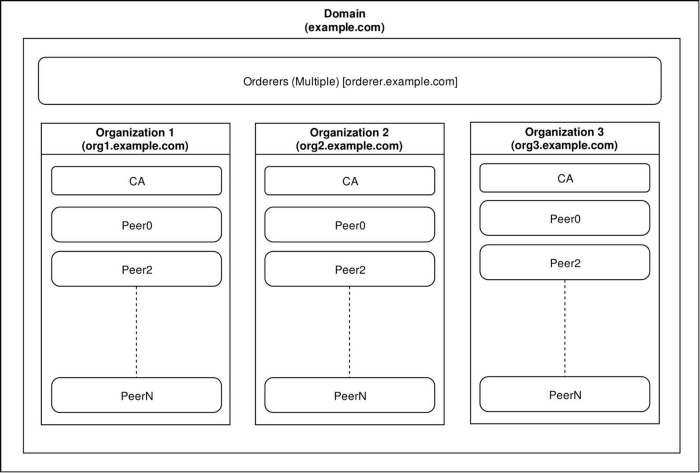
\includegraphics[width=1\linewidth]{pictures/hyperledger-fabric-architecture}
	\caption[Hyperledger Fabric Architecture]{Hyperledger Fabric Architecture (eigene Darstellung)}
	\label{fig:hyperledger-fabric-architecture}
\end{figure}

\subsection{Zusammenfassung Systementwurf}
1. Anforderungsschema wurde beschrieben\\
2. Ziele wurden erläutert\\
3. Wertschöpfungskette und Geschäftsprozesse wurden dargestellt\\
4. Rahmenbedingungen und Qualitätsanforderungen wurden beschrieben\\
5. Funktionale Anforderungen wurden festgehalten\\
6. Systementwurf wurde dokumentiert\\
7. Ausblick nächstes Kapitel auf konkrete technische Umsetzung

\newpage
